\chapter{Results}
\label{ch:results}

This chapter reports the experimental outcomes of the classification pipeline described in \Cref{ch:classification}, evaluated under Leave-One-Run-Out cross-validation (LORO-CV, \Cref{sec:eval_protocol}) on three classification problems: the five-class campus development dataset (Dataset~A, \Cref{sec:initial_dev_dataset}), its three-class low-constant-speed subset (Dataset~B), and the primary three-class farm dataset (\Cref{sec:farm_dataset}). Headline figures of merit are the macro-averaged $F_1$ score and the robustness score $r = \overline{F_1^{\mathrm{macro}}} - 0.5\,\sigma_{F_1^{\mathrm{macro}}}$ defined in \Cref{eq:robustness}. \Cref{sec:res_campus,sec:res_farm} present the per-dataset findings. \Cref{sec:res_speed} isolates the velocity--vibration confound discussed in \Cref{sec:bg-vel} by comparing the multi-speed and low-speed campus subsets.\Cref{sec:res_models} cross-cuts the model families and adds the robustness diagnostics (sensor dropout, noise injection, cross-day variation, significance testing). \Cref{sec:res_transition} finally evaluates the sliding-window classifier as a transition detector, both with the implicit $n_{\text{stable}}$ stable-run rule and with the CUSUM detector whose formulation is given in \Cref{sec:bg-transition}.

\section{Test Dataset: Campus Development Route}
\label{sec:res_campus}

The campus dataset was recorded to develop the pipeline against varied outdoor surfaces before the farm campaign (\Cref{sec:initial_dev_dataset}). It is evaluated here in three nested configurations, each of which isolates a single source of difficulty:
\begin{itemize}
    \item \emph{Dataset~A (5-class)} --- all windows, all five labels (\texttt{grass}, \texttt{smooth\_terrain}, \texttt{dry\_dirt\allowbreak \_track}, \texttt{muddy\_dirt\_track}, \texttt{cobblestone}). The full multi-speed problem with the two rare classes still in place. All six classifier families (LR, RF, XGBoost, SVM, MLP, CNN) are evaluated.
    \item \emph{Dataset~A (3-class)} --- the same multi-speed windows but restricted to the three classes that are well populated across every session (\texttt{grass}, \texttt{smooth\_terrain}, \texttt{dry\_\allowbreak dirt\_track}). Compared to the 5-class problem, this configuration changes \emph{only} the class set: the speed range and the windowing protocol are identical. Only the four classical baselines (LR, RF, XGBoost, SVM) are evaluated on this configuration, since it serves purely as a controlled comparison point for isolating the class-imbalance effect from the speed-regime effect.
    \item \emph{Dataset~B (3-class)} --- the same three classes, further restricted to the low-constant-speed regime selected by \Cref{eq:dataset_B_mask}. Because the campus robot was already operated at a moderate speed most of the time, Dataset~B sits inside Dataset~A: more than $75\,\%$ of the 3-class Dataset~A windows already satisfy the speed mask. It also provides a more parallel comparison point with the farm dataset (\Cref{sec:res_farm}), since the class count and speed regime match. All six classifier families are evaluated.
\end{itemize}

\paragraph{Dataset~A, 5 classes --- the full problem.} \Cref{tab:campus_master} lists the best configuration of each classifier family on the full five-class Dataset~A. The six families fall within a narrow $F_1^{\mathrm{macro}}$ band of $0.728$ (SVM) to $0.766$ (MLP), a spread of $\sim 0.04$ that is substantially smaller than the cross-fold standard deviation $\sigma_{F_1} \approx 0.12$--$0.15$ within each family. The paired Wilcoxon test on the per-fold scores (\Cref{fig:significance_campus}) returns no pair with $p < 0.05$, so no model family is statistically distinguishable from another at the $5\,\%$ level. The stratified-dummy baseline scores $0.20$ macro-$F_1$ against the $0.20$ chance level for five classes, confirming that the LORO splits do not themselves leak class structure. The cross-fold variance is itself driven mostly by the two rare classes discussed next.

\begin{table}[H]
\centering
\caption{Best configuration of each classifier family on the five-class campus Dataset~A under LORO-CV. \texttt{Config} is the (feature-set, imbalance-handling) selection. The CNN consumes raw $5 \times 200$ windows and has no feature-set choice.} % Source: \texttt{results/Campus/master\_model\_comparison.csv}.}
\label{tab:campus_master}
\begin{tabular}{llccc}
\toprule
\textbf{Model} & \textbf{Config} & $\overline{F_1}$ & 95\% CI &
\textbf{Worst fold} \\
\midrule
MLP                & \texttt{top\_mi}            & 0.766 & $\pm 0.165$ & 0.599 \\
LogisticRegression & \texttt{all, balanced}      & 0.765 & $\pm 0.151$ & 0.626 \\
XGBoost            & \texttt{top\_mi, balanced}  & 0.765 & $\pm 0.178$ & 0.579 \\
RandomForest       & \texttt{all, unweighted}    & 0.759 & $\pm 0.152$ & 0.609 \\
CNN                & raw signal (5\,ch)          & 0.757 & $\pm 0.191$ & 0.567 \\
SVM                & \texttt{top\_mi, balanced}  & 0.728 & $\pm 0.134$ & 0.636 \\
\midrule
Dummy (stratified) & ---                         & 0.201 & $\pm 0.031$ & 0.174 \\
\bottomrule
\end{tabular}
\end{table}

\begin{figure}[H]
    \centering
    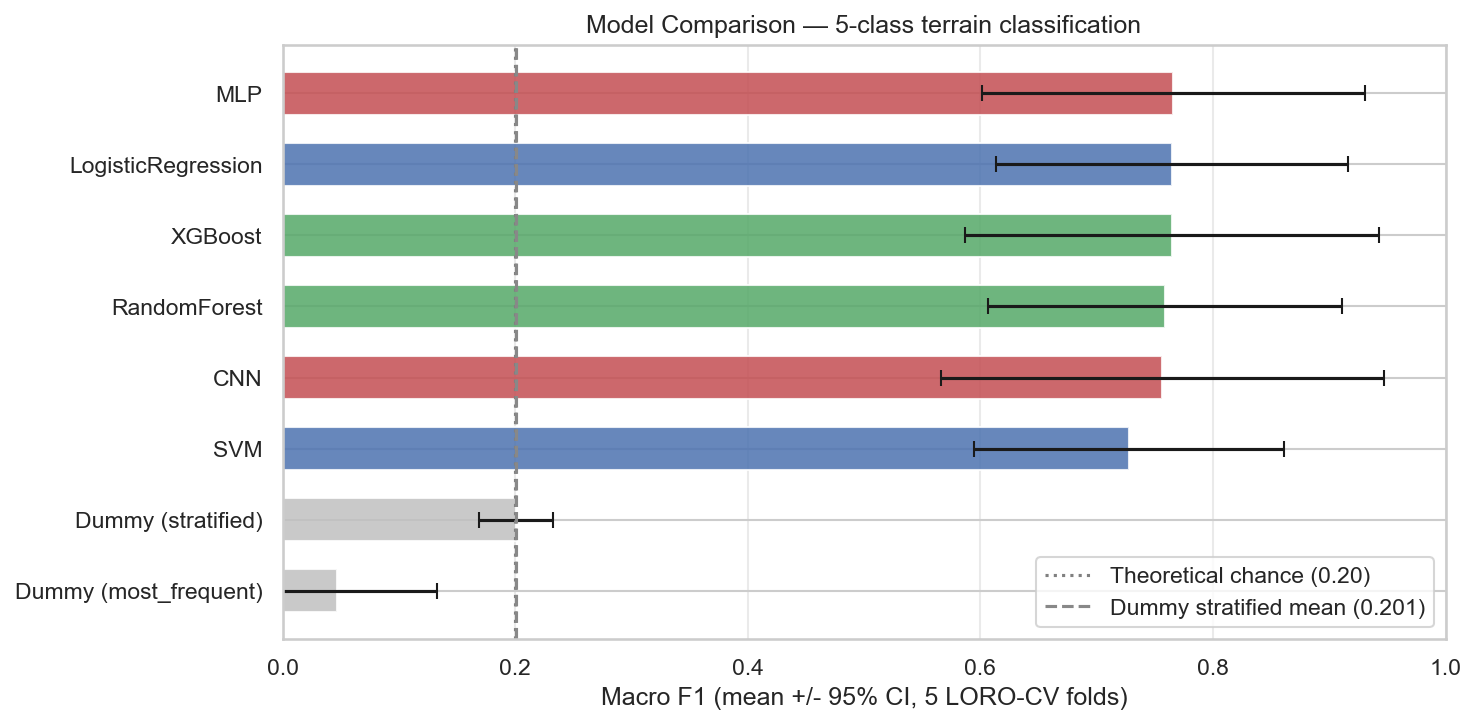
\includegraphics[width=\textwidth]{Pictures/Figures/master_comparison_C5.png}
    \caption{Master model comparison on the five-class campus Dataset~A.}
    \label{fig:campus_master_bars}
\end{figure}

\paragraph{Per-class failures driven by class imbalance and route effects.} The aggregate $F_1 \approx 0.77$ headline number on Dataset~A is heavily diluted by two minority classes whose per-class scores collapse on the worst folds. \Cref{tab:campus_perclass} summarises the per-class XGBoost numbers; the picture is essentially the same for the other classical models. \texttt{Cobblestone} reaches only $F_1 = 0.33$, with one fold scoring $0.04$ and the other $0.62$. \texttt{Muddy\_dirt\_track} fares only marginally better, at $F_1 = 0.44$ with a high recall variance and a worst-fold value of $0.10$. The fold-quality diagnostic %TODO: ADD THE TABLE IN THE APPENDIX AND REFER TO THAT INSTEAD
(\texttt{results/Campus/fold\_quality\_diagnostics.csv}) explains the collapse: both classes are recorded almost exclusively on a single session each (cobblestone on Run~B of the 9~March log and on the 26~March log; muddy dirt track on the two snowy February sessions), so when the dominant run becomes the test fold the model has essentially no training data for that class and has to predict the next-closest category. Speed conditioning aggravates the same problem: every speed-imbalanced minority class is flagged with a speed total-variation distance of $0.56$--$0.86$ between train and test in the diagnostic table. The behaviour is therefore not a model failure but a dataset-collection limitation, and is what motivates dropping the two classes in the next configuration.

\begin{table}[H]
\centering
\caption{Per-class XGBoost ($F_1$) on the five-class campus Dataset~A. \texttt{folds\_evaluated} is the number of folds in which the class appears in both train and test partitions.}
\label{tab:campus_perclass}
\begin{tabular}{lcccc}
\toprule
\textbf{Class} & $\overline{F_1}$ & $\sigma_{F_1}$ &
\textbf{Worst} & \textbf{Folds} \\
\midrule
smooth\_terrain        & 0.947 & 0.026 & 0.912 & 5 \\
dry\_dirt\_track       & 0.895 & 0.018 & 0.877 & 2 \\
grass                  & 0.863 & 0.105 & 0.693 & 5 \\
muddy\_dirt\_track     & 0.436 & 0.339 & 0.096 & 2 \\
cobblestone            & 0.329 & 0.292 & 0.037 & 2 \\
\bottomrule
\end{tabular}
\end{table}

\begin{figure}[H]
    \centering
    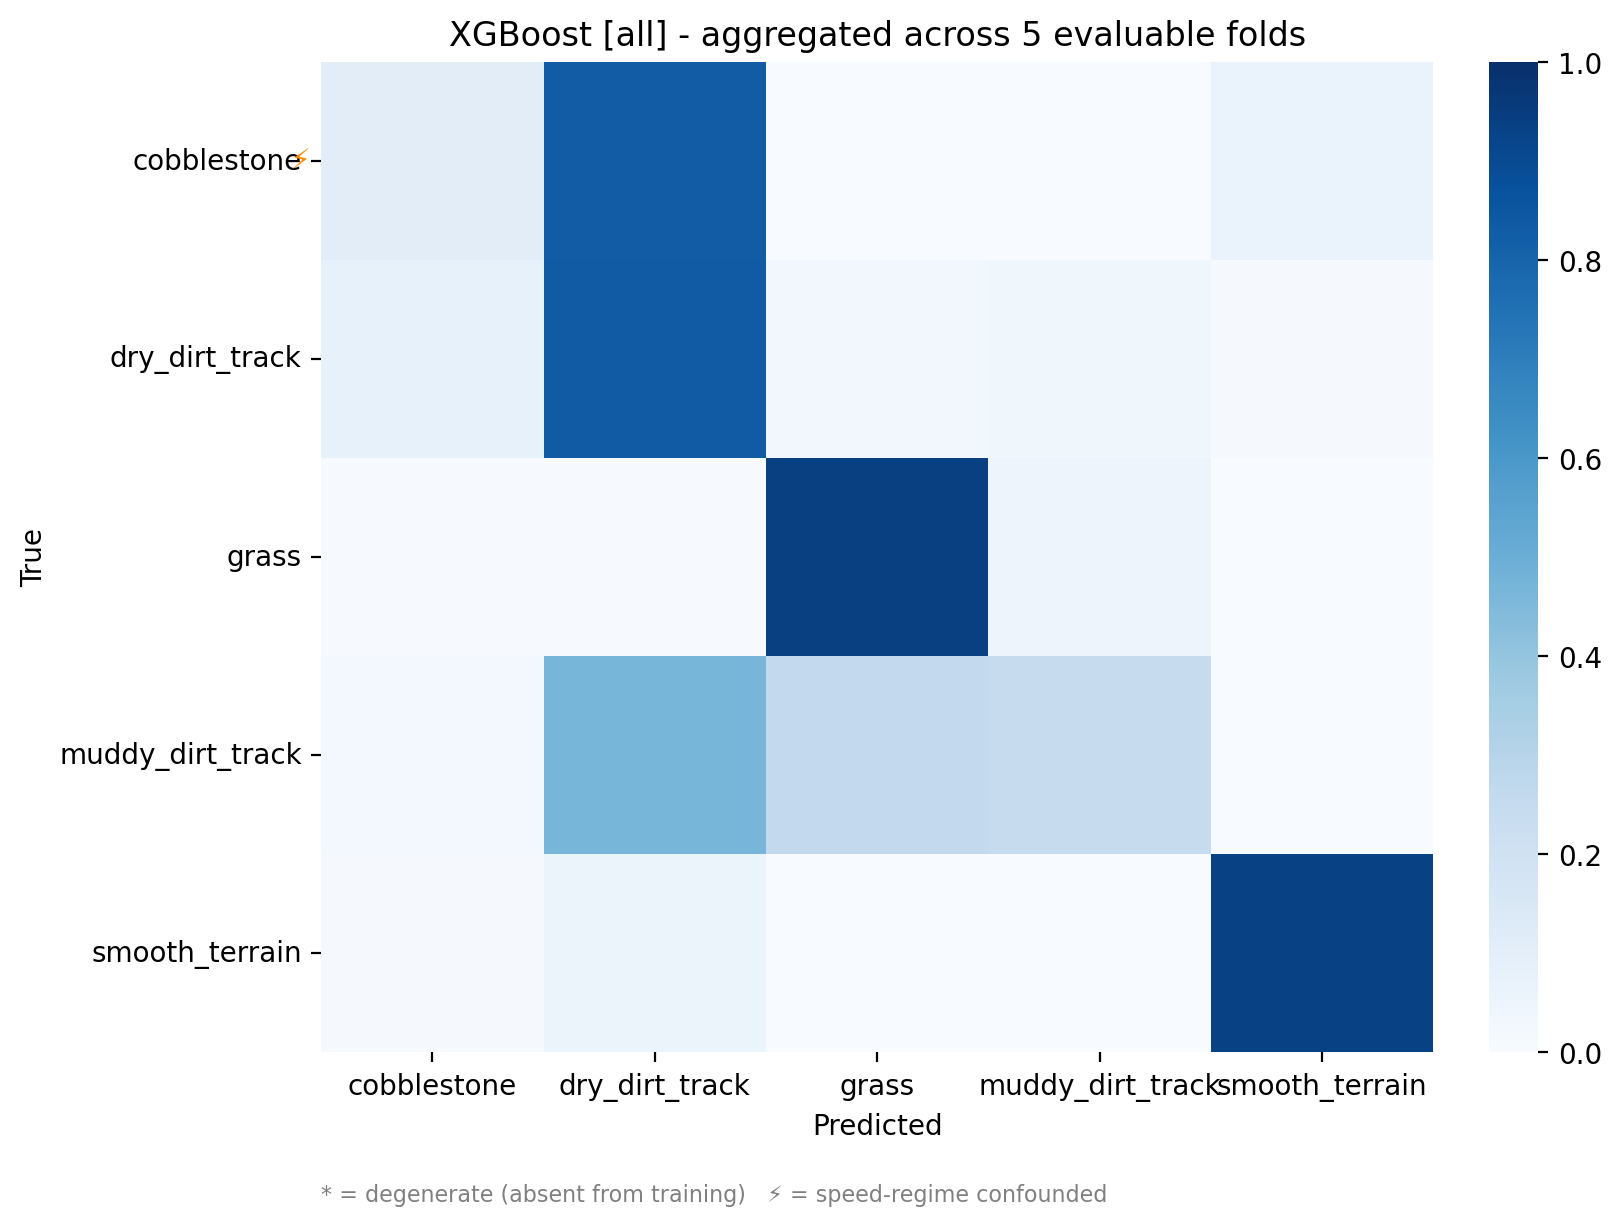
\includegraphics[width=\textwidth]{Pictures/Figures/confusion_matrix_xgboost_all_C5.png}
    \caption{Aggregated XGBoost confusion matrix on the five-class campus Dataset~A. The minority classes \texttt{cobblestone} and \texttt{muddy\_dirt\_track} are systematically confused with the larger-class neighbours of similar roughness.}
    \label{fig:campus_cm_5class}
\end{figure}

\paragraph{Dataset~A, 3 classes --- isolating the class-imbalance effect.} \label{par:campus_a_3class} Re-running every classical classifier on the same multi-speed Dataset~A, but with the two collapsing minority classes removed, recovers a much higher headline performance. \Cref{tab:campus_A_3class} shows that every classical model now exceeds $F_1 = 0.94$ and reaches $0.96$--$0.97$ in its best configuration. The 5-class to 3-class delta on the \emph{same windows and the same speed range} is therefore $\sim 0.20$ macro-$F_1$ better for every model family (\Cref{tab:campus_5cls_to_3cls_delta}). This number is the cleanest available estimate of how much of the campus 5-class difficulty is attributable to the two rare classes alone: nothing about the model, the features or the speed regime has changed between the two rows of \Cref{tab:campus_5cls_to_3cls_delta}, only the label set.

\begin{table}[H]
\centering
\caption{Best configuration of each classifier on the three-class campus Dataset~A.}% Source: \texttt{results/Campus/dataset\_A\_3class\_metrics\_summary.csv}.}
\label{tab:campus_A_3class}
\begin{tabular}{llccc}
\toprule
\textbf{Model} & \textbf{Config} & $\overline{F_1}$ & 95\% CI &
\textbf{Worst fold} \\
\midrule
LogisticRegression & \texttt{top\_mi, balanced}    & 0.974 & $\pm 0.018$ & 0.952 \\
XGBoost            & \texttt{all, balanced}        & 0.968 & $\pm 0.029$ & 0.937 \\
RandomForest       & \texttt{all, unweighted}      & 0.960 & $\pm 0.025$ & 0.928 \\
SVM                & \texttt{top\_mi, balanced}    & 0.975 & $\pm 0.014$ & 0.956 \\
\bottomrule
\end{tabular}
\end{table}

\begin{table}[H]
\centering
\caption{Effect of dropping the two minority classes from the campus dataset. Both rows use the same multi-speed windows and the same \texttt{balanced} configuration; only the label set differs.}% Source: \texttt{results/Campus/comparison\_3class\_vs\_5class\_multispeed.csv}.}
\label{tab:campus_5cls_to_3cls_delta}
\begin{tabular}{lcccc}
\toprule
\textbf{Model} & \textbf{5-class (A)} & \textbf{3-class (A)} & $\Delta F_1$ \\
\midrule
LogisticRegression & 0.760 & 0.967 & $+0.207$ \\
XGBoost            & 0.768 & 0.958 & $+0.190$ \\
RandomForest       & 0.749 & 0.952 & $+0.203$ \\
SVM                & 0.727 & 0.946 & $+0.219$ \\
\bottomrule
\end{tabular}
\end{table}

\paragraph{Dataset~B, 3 classes --- isolating the speed-regime effect.} Applying the low-constant-speed mask of \Cref{eq:dataset_B_mask} on top of the 3-class label set produces Dataset~B. Because more than $75\,\%$ of the 3-class Dataset~A windows already satisfy that mask, Dataset~B is a slight trim rather than a different dataset: any difference in the headline number is the residual effect of removing the high-speed and accelerating windows on an otherwise identical problem. \Cref{tab:campus_A3_vs_B3} reports the A~(3-class)~$\to$~B paired comparison: every classical model gains $0.005$--$0.026$ macro-$F_1$ in the low-speed regime, the direction of the gain is consistent across all four families, and the worst-fold $F_1$ also improves. The gain is, however, an order of magnitude smaller than the $\sim 0.20$ improvement from dropping the minority classes, so on this dataset the class-imbalance effect appears to contribute more to the headline gap than the speed regime does. This reading should be qualified, however: because Dataset~B contains the majority of the Dataset~A~(3-class) windows, the paired comparison only measures the marginal contribution of the $\sim 25\,\%$ of windows that the speed mask removes, and the speed range present on the campus logs is itself bounded by the driving profile of those sessions. A stronger statement about the velocity-vibration confound of \Cref{sec:bg-vel} would require a dedicated experiment recording the same surfaces over a deliberately wide speed range; from the present data alone, the safe conclusion is the weaker one that the speed effect is real, consistent in direction across model families, and small in magnitude at the operating point sampled here.

\Cref{tab:campusB_master} lists the absolute Dataset~B numbers: every classifier family now exceeds $F_1 = 0.95$, with SVM and Logistic Regression reaching $0.986$ and $0.984$ respectively, and the fold-to-fold standard deviation drops by an order of magnitude relative to Dataset~A.

\begin{table}[H]
\centering
\caption{Three-class campus problem at the multi-speed (Dataset~A) and low-constant-speed (Dataset~B) regimes, balanced configurations. $\Delta F_1$ = B $-$ A. Because Dataset~B is a strict subset of Dataset~A, this is a direct paired comparison of the speed-regime effect on an otherwise identical problem.}% Source: \texttt{results/Campus/dataset\_A\_3class\_vs\_B\_3class\_contextual\_comparison.csv}.}
\label{tab:campus_A3_vs_B3}
\begin{tabular}{lccc}
\toprule
\textbf{Model} & \textbf{A (3-cls, multi-speed)} & \textbf{B (3-cls, low-speed)} & $\Delta F_1$ \\
\midrule
LogisticRegression & 0.967 & 0.970 & $+0.003$ \\
SVM                & 0.946 & 0.958 & $+0.012$ \\
RandomForest       & 0.952 & 0.978 & $+0.026$ \\
XGBoost            & 0.958 & 0.979 & $+0.021$ \\
\bottomrule
\end{tabular}
\end{table}

\begin{table}[H]
\centering
\caption{Best configuration of each classifier family on the three-class campus Dataset~B.}% Source: \texttt{results/Campus\_dataset\_B\_3class/master\_model\_comparison.csv}.}
\label{tab:campusB_master}
\begin{tabular}{llccc}
\toprule
\textbf{Model} & \textbf{Config} & $\overline{F_1}$ & 95\% CI &
\textbf{Worst fold} \\
\midrule
SVM                & \texttt{top\_mi, balanced}   & 0.986 & $\pm 0.030$ & 0.957 \\
LogisticRegression & \texttt{top\_mi, balanced}   & 0.984 & $\pm 0.020$ & 0.966 \\
RandomForest       & \texttt{top\_mi, unweighted} & 0.983 & $\pm 0.033$ & 0.952 \\
XGBoost            & \texttt{top\_mi, unweighted} & 0.982 & $\pm 0.023$ & 0.961 \\
MLP                & \texttt{top\_mi}             & 0.965 & $\pm 0.058$ & 0.912 \\
CNN                & raw signal (5\,ch)           & 0.952 & $\pm 0.081$ & 0.902 \\
\bottomrule
\end{tabular}
\end{table}

\begin{figure}[H]
    \centering
    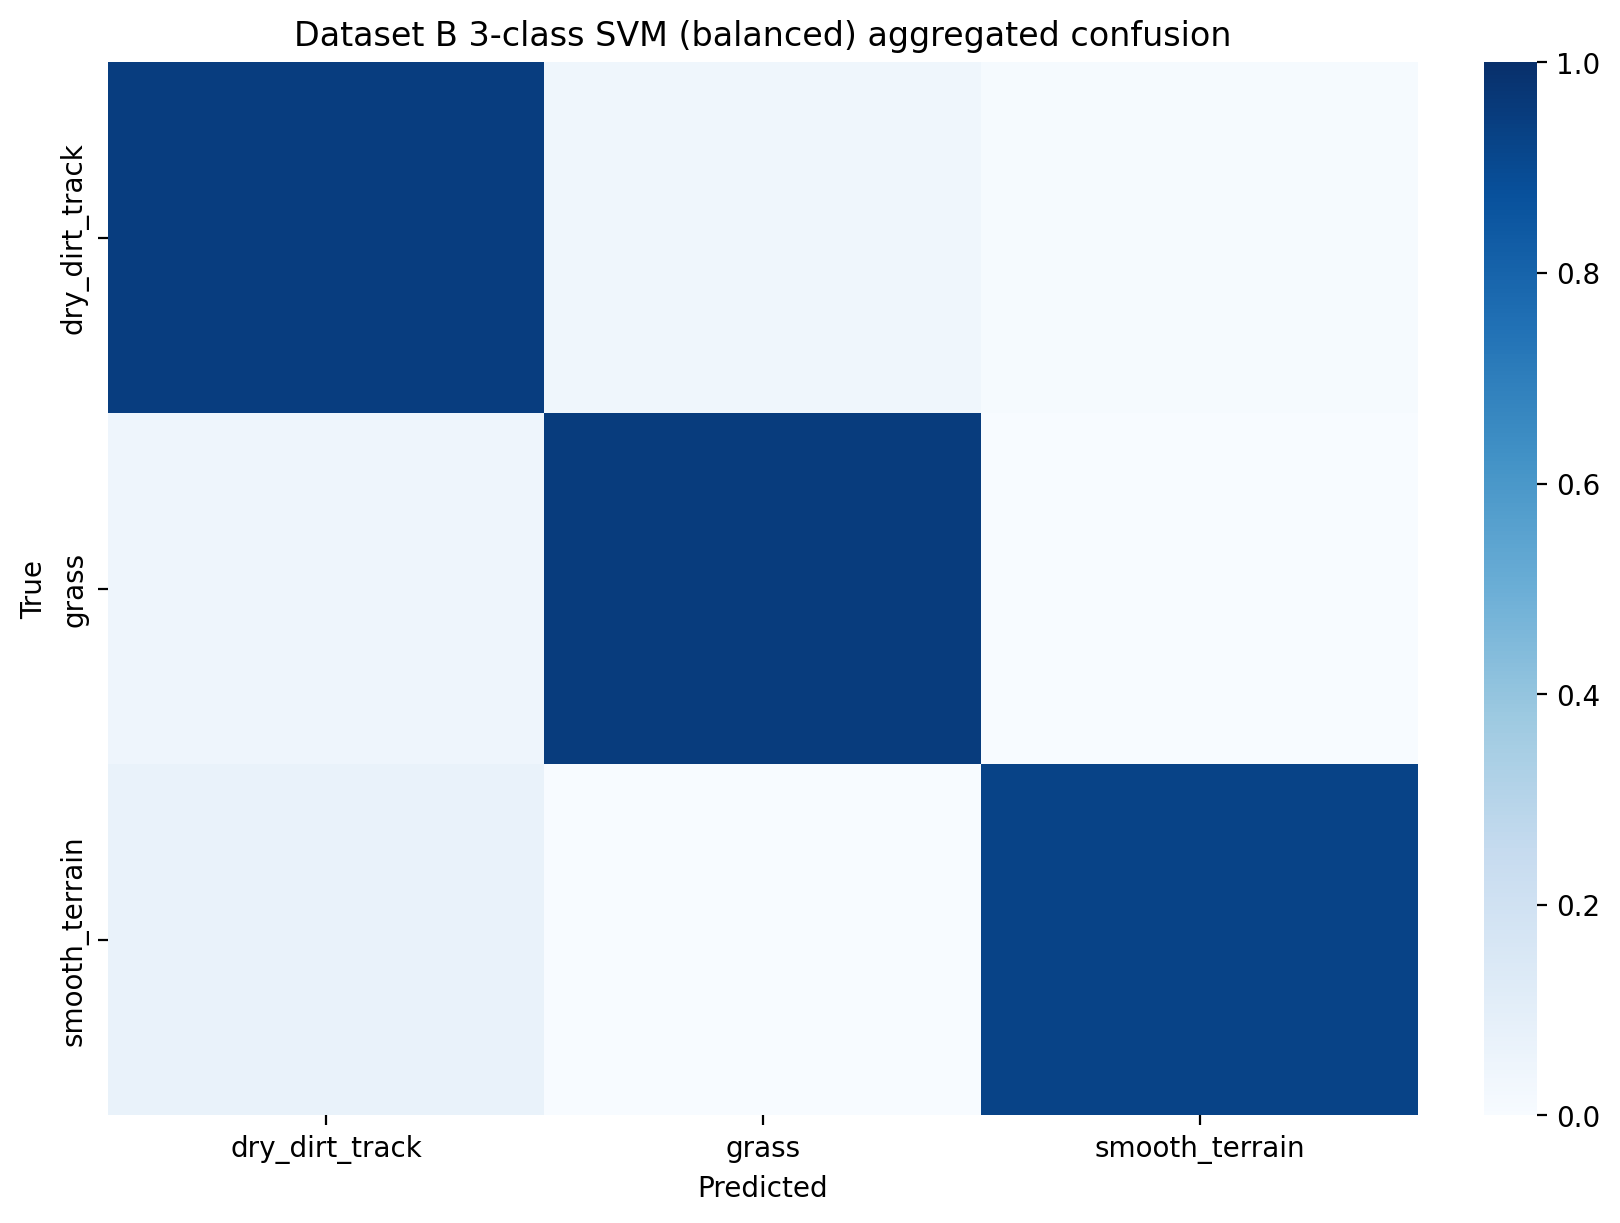
\includegraphics[width=\textwidth]{Pictures/Figures/confusion_matrix_svm_aggregated.png}
    \caption{Aggregated SVM confusion matrix on the three-class campus Dataset~B. Off-diagonal mass is below $5\,\%$ in every cell, illustrating that the residual errors are not class-specific.}
    \label{fig:campusB_cm_3class}
\end{figure}

\begin{figure}[H]
    \centering
    \placeholder{Insert a three-bar figure (one bar per dataset
    configuration) showing macro-$F_1$ at A~(5-class), A~(3-class), B~(3-class)
    for a representative classifier (e.g.\ XGBoost \texttt{balanced}). The
    big step is between bars 1 and 2; bar 3 is only marginally higher than
    bar 2. Data sources:
    \texttt{master\_model\_comparison.csv},
    \texttt{dataset\_A\_3class\_metrics\_summary.csv}, and
    \texttt{Campus\_dataset\_B\_3class/master\_model\_comparison.csv}.}
    \caption{Decomposition of the campus headline number: the
    A~(5-class)~$\to$~A~(3-class) jump (class-imbalance effect) is roughly
    ten times larger than the A~(3-class)~$\to$~B~(3-class) jump
    (speed-regime effect).}
    \label{fig:campus_decomposition}
\end{figure}

\paragraph{Reading the three configurations together.}
The three-configuration sweep separates the two sources of headline
improvement that were entangled in the 5-class~$\to$~B comparison. Dropping
the minority classes is worth $\sim 0.20$ macro-$F_1$ on the same
multi-speed windows; restricting to the low-constant-speed regime on top of
that buys a further $\sim 0.01$--$0.026$. The Dataset~B headline of
$F_1 = 0.98$ is therefore not a meaningful improvement of the method; it is
a near-saturated reference point that says \emph{how easy a three-class
campus problem becomes once the dataset itself is sufficient}. The farm
dataset analysed next is the more realistic operating point, and the
$\sim 0.12$ gap between the Dataset~B campus result and the farm result is
attributable to the harder class structure of the farm
(\texttt{grass}--\texttt{soil} confusion) rather than to a residual
speed effect.

\section{Farm Dataset: Primary Classification Result}
\label{sec:res_farm}

The farm dataset is the primary target of this thesis: three terrain classes
(\texttt{dirt\_track}, \texttt{grass}, \texttt{soil}) recorded across five
runs on two field days under broadly consistent weather and at the
intrinsically low and roughly constant speed at which the platform operates
in production (\Cref{sec:farm_dataset}).

\paragraph{Headline performance.}
\Cref{tab:farm_master} lists the best configuration of each classifier
family. The three top classical baselines (SVM, Logistic~Regression,
XGBoost) achieve $F_1 \approx 0.86$ and overlap within their $95\,\%$ CIs.
The CNN, which sees only the raw five-channel windowed signal, comes within
$\sim 0.02$ of the engineered-feature baselines despite a markedly larger
cross-fold spread. The MLP and the random forest sit slightly behind. The
paired Wilcoxon test
(\Cref{fig:significance_farm}, source
\texttt{results/Farm/significance\_pvalues.csv}) returns no model pair with
$p < 0.05$, so the ordering in \Cref{tab:farm_master} is best read as a
single $0.84$--$0.86$ macro-$F_1$ cluster rather than a strict ranking.

\begin{table}[H]
\centering
\caption{Best configuration of each classifier family on the three-class
farm dataset under LORO-CV. Source:
\texttt{results/Farm/master\_model\_comparison.csv}.}
\label{tab:farm_master}
\begin{tabular}{llccc}
\toprule
\textbf{Model} & \textbf{Config} & $\overline{F_1}$ & 95\% CI &
\textbf{Worst fold} \\
\midrule
SVM                & \texttt{all, unweighted}   & 0.866 & $\pm 0.075$ & 0.813 \\
LogisticRegression & \texttt{all, unweighted}   & 0.865 & $\pm 0.084$ & 0.786 \\
XGBoost            & \texttt{all, balanced}     & 0.861 & $\pm 0.060$ & 0.823 \\
CNN                & raw signal (5\,ch)         & 0.849 & $\pm 0.100$ & 0.721 \\
MLP                & \texttt{all}               & 0.840 & $\pm 0.088$ & 0.746 \\
RandomForest       & \texttt{all, unweighted}   & 0.840 & $\pm 0.059$ & 0.794 \\
\midrule
Dummy (stratified) & ---                        & 0.320 & $\pm 0.013$ & 0.305 \\
\bottomrule
\end{tabular}
\end{table}

\begin{figure}[H]
    \centering
    \placeholder{Insert \texttt{reports/models/Farm/master\_comparison.png}.}
    \caption{Master model comparison on the farm dataset. The
    classical, MLP and CNN families overlap within a single cluster
    centred on $F_1 \approx 0.85$.}
    \label{fig:farm_master_bars}
\end{figure}

\paragraph{Per-class structure: \texttt{grass} is the hard one.}
\Cref{tab:farm_perclass} shows that the residual error on the farm dataset is
concentrated in the \texttt{grass} class, which scores $F_1 = 0.74$ against
$0.85$ for \texttt{soil} and $0.98$ for \texttt{dirt\_track}. The aggregated
confusion matrix (\Cref{fig:farm_cm}) shows that \texttt{grass} is most often
mistaken for \texttt{soil}: short grass on firm soil and bare loose soil
produce visually and proprioceptively similar low-amplitude, low-frequency
chassis motion, and the cross-sensor correlations selected by the MI ranking
(\Cref{sec:feat_mi_pruning}) are not always enough to separate them on a
single run. \texttt{Dirt\_track} is essentially solved on every fold, which
is consistent with the physical picture: a compacted track produces a
high-amplitude, broad-spectrum vibration signature that the other two
classes do not exhibit.

\begin{table}[H]
\centering
\caption{Per-class XGBoost ($F_1$) on the farm dataset. All three classes
are evaluable in every fold. Source:
\texttt{results/Farm/per\_class\_metrics\_xgboost.csv}.}
\label{tab:farm_perclass}
\begin{tabular}{lcccc}
\toprule
\textbf{Class} & $\overline{F_1}$ & $\sigma_{F_1}$ &
\textbf{Worst} & \textbf{Folds} \\
\midrule
dirt\_track & 0.976 & 0.027 & 0.922 & 5 \\
soil        & 0.848 & 0.065 & 0.789 & 5 \\
grass       & 0.744 & 0.116 & 0.562 & 5 \\
\bottomrule
\end{tabular}
\end{table}

\begin{figure}[H]
    \centering
    \placeholder{Insert
    \texttt{reports/models/Farm/confusion\_matrix\_xgboost\_all.png}.
    Aggregated three-class XGBoost confusion matrix.}
    \caption{Aggregated XGBoost confusion matrix on the farm dataset.
    \texttt{Grass} confusion mass is concentrated on \texttt{soil};
    \texttt{dirt\_track} is essentially separable.}
    \label{fig:farm_cm}
\end{figure}

\paragraph{Cross-day robustness.}
The five farm runs span two field days
(\Cref{tab:farm_sessions}), and the per-run macro-$F_1$ values
(\Cref{tab:farm_crossday}) drop systematically from day~1 (Run1,~Run2) to
day~2 (Run3--Run5) across every model family. Day~1 averages
$F_1 \approx 0.92$ while day~2 averages $F_1 \approx 0.83$ --- a $\sim 0.09$
point gap that is consistent across all six families and that exceeds the
fold-to-fold variation within a single day. The two days share weather,
robot, route plan, and labelling protocol, so the residual variation is
attributable to changes in soil moisture, grass blade density and the
operator-driven within-day route choice. The same plateau pattern shows up
on the campus dataset (\Cref{fig:campus_crossday}), where the gap is
substantially larger because the weather conditions vary between sessions.

\begin{table}[H]
\centering
\caption{Per-run macro-$F_1$ on the farm dataset, three top models. Day~1 =
21~Apr~2026 (Run1,~Run2); day~2 = 28~Apr~2026 (Run3,~Run4,~Run5). Source:
\texttt{results/Farm/cross\_day\_performance.csv}.}
\label{tab:farm_crossday}
\begin{tabular}{lccccc}
\toprule
\textbf{Model} & Run1 & Run2 & Run3 & Run4 & Run5 \\
\midrule
SVM                & 0.958 & 0.895 & 0.832 & 0.813 & 0.830 \\
LogisticRegression & 0.972 & 0.864 & 0.846 & 0.786 & 0.859 \\
XGBoost            & 0.940 & 0.876 & 0.836 & 0.829 & 0.823 \\
\bottomrule
\end{tabular}
\end{table}

\begin{figure}[H]
    \centering
    \placeholder{Insert
    \texttt{reports/models/Farm/cross\_day\_performance.png}.}
    \caption{Per-run macro-$F_1$ on the farm dataset. The day-1/day-2 step
    is consistent across all six model families.}
    \label{fig:farm_crossday}
\end{figure}

\begin{figure}[H]
    \centering
    \placeholder{Insert
    \texttt{reports/models/Campus/cross\_day\_performance.png}.}
    \caption{Per-session macro-$F_1$ on the campus dataset. Inter-session
    variation here is dominated by weather changes (snow/rain in the
    February sessions vs.\ dry pavement in March).}
    \label{fig:campus_crossday}
\end{figure}

\paragraph{Sensor-dropout robustness.}
\label{par:sensor_dropout}
A central question for an intrinsic-only terrain pipeline is which of the
three sensor channel groups --- accelerometer, gyroscope, and odometry ---
actually carries the discriminative information, and how gracefully the
pipeline degrades if one of them fails. Each channel group was disabled
in two modes (\Cref{tab:dropout_farm}): (i)~\emph{test-time zero},
simulating a transient sensor failure at deployment by zero-ing the
corresponding columns on the held-out fold only (the model was trained on
the full feature table), and (ii)~\emph{full ablation}, simulating a
permanent removal at design time by retraining the model without those
columns. The contrast between the two is informative: a sensor that is
catastrophic at (i) but harmless at (ii) is one the model has learned to
rely on; a sensor that is harmless at both is one whose information was
redundant from the start.

\begin{table}[H]
\centering
\caption{Sensor-dropout robustness on the farm dataset (LogisticRegression).
$\Delta F_1$ is measured against the all-features baseline of
$F_1 = 0.842$. Source: \texttt{results/Farm/sensor\_dropout.csv}.}
\label{tab:dropout_farm}
\begin{tabular}{llcc}
\toprule
\textbf{Channel group} & \textbf{Mode} & $\overline{F_1}$ &
$\Delta F_1$ \\
\midrule
All features (baseline) & ---                    & 0.842 & $0.000$ \\
Accelerometer           & test-time zero         & 0.515 & $-0.328$ \\
Accelerometer           & full ablation (retrain)& 0.818 & $-0.024$ \\
Gyroscope               & test-time zero         & 0.579 & $-0.263$ \\
Gyroscope               & full ablation (retrain)& 0.837 & $-0.005$ \\
Odometry                & test-time zero         & 0.841 & $-0.001$ \\
Odometry                & full ablation (retrain)& 0.843 & $+0.000$ \\
\bottomrule
\end{tabular}
\end{table}

Two findings stand out. First, a transient loss of \emph{either} the
accelerometer or the gyroscope on the farm dataset is catastrophic
(test-time-zero $\Delta F_1$ of $-0.33$ and $-0.26$ respectively), but a
permanent loss is essentially recoverable by retraining ($\Delta F_1$ of
$-0.02$ and $-0.01$). The model can express the terrain signature equally
well in either inertial channel \emph{group} alone --- pitch/roll rates and
the vertical accelerometer share the same physical excitation --- but if it
has been trained on both and then loses one without warning, the standardised
zero values land far outside the in-distribution feature space and the
classifier's decision boundary breaks. Second, odometry is essentially free:
neither the test-time zero nor the full ablation moves $F_1$ by more than
$0.001$. The discriminative information was already absorbed by the
speed-normalised vibration features, and the explicit odometry columns do
not add a separable contribution on top.

\begin{figure}[H]
    \centering
    \placeholder{Insert \texttt{reports/models/Farm/sensor\_dropout.png}.
    Grouped bar chart of $\Delta F_1$ for the six (sensor, mode)
    combinations vs.\ the all-features baseline, with CI error bars.}
    \caption{Sensor-dropout robustness on the farm dataset. The contrast
    between the test-time-zero columns and the full-ablation columns
    indicates that the model can express the terrain signature in any
    one inertial channel alone, but it cannot tolerate a silent failure
    of a channel it was trained on.}
    \label{fig:dropout_farm}
\end{figure}

The campus picture is markedly different
(\Cref{tab:dropout_campus_compare}). On the five-class Dataset~A, zeroing
the gyroscope at test time costs $\Delta F_1 = -0.39$ while zeroing the
accelerometer costs only $-0.12$, and on the three-class Dataset~B the
asymmetry sharpens to $-0.62$ vs $-0.007$. The gyroscope is dominant on
campus and roughly co-equal with the accelerometer on the farm. The most
plausible explanation lies in the surface mix: the campus dataset includes
extremes of stiffness (smooth asphalt vs cobblestone) whose discriminative
signature is dominated by the pitch and roll modes that the gyroscope
captures, whereas the farm classes (\texttt{dirt\_track}, \texttt{soil},
\texttt{grass}) differ as much in vertical-acceleration amplitude as in
chassis-rocking, so the discriminative information is split more evenly
across the two inertial sensor groups. The campus-B accelerometer ablation
that costs essentially nothing ($-0.007$) is consistent with the same
picture --- on a three-class problem dominated by pitch/roll signatures the
accelerometer is redundant.

\begin{table}[H]
\centering
\caption{Test-time-zero sensor dropout across all three datasets, expressed
as $\Delta F_1$ against the all-features baseline. Source:
\texttt{results/comparison/master\_model\_comparison\_farm\_vs\_campus.csv}
and the per-dataset \texttt{sensor\_dropout.csv} files.}
\label{tab:dropout_campus_compare}
\begin{tabular}{lccc}
\toprule
\textbf{Channel zeroed} & \textbf{Farm (3-cls)} &
\textbf{Campus A (5-cls)} & \textbf{Campus B (3-cls)} \\
\midrule
Accelerometer & $-0.328$ & $-0.118$ & $-0.007$ \\
Gyroscope     & $-0.263$ & $-0.387$ & $-0.616$ \\
Odometry      & $-0.001$ & $-0.011$ & $-0.002$ \\
\bottomrule
\end{tabular}
\end{table}

\begin{figure}[H]
    \centering
    \placeholder{Insert
    \texttt{reports/models/comparison/sensor\_dropout\_farm\_vs\_campus.png}.}
    \caption{Sensor-dropout comparison across the three datasets. The
    accelerometer/gyroscope balance is roughly even on the farm but
    strongly gyroscope-skewed on the campus, particularly on the
    three-class subset.}
    \label{fig:dropout_compare}
\end{figure}

\paragraph{Noise sensitivity.}
\Cref{fig:noise_sensitivity} shows the macro-$F_1$ degradation when zero-mean
Gaussian noise of standard deviation $\sigma$ (in units of the standardised
feature) is added to the test fold only. The farm dataset degrades
gracefully from $0.84$ at $\sigma = 0$ to $0.59$ at $\sigma = 2.0$; the
five-class campus drops more steeply, from $0.75$ to $0.39$, while the
three-class campus subset starts the highest ($0.86$) and ends at $0.47$.
The crossover at $\sigma \approx 0.8$ between Campus~A and Campus~B reflects
the fact that the high baseline of Dataset~B is partly carried by a
narrow-margin SVM that is more easily disrupted than the broader
feature-space decision boundary on Dataset~A.

\begin{figure}[H]
    \centering
    \placeholder{Insert
    \texttt{reports/models/comparison/noise\_sensitivity\_farm\_vs\_campus.png}.}
    \caption{Noise sensitivity across the three datasets. The farm
    classifier degrades the most gracefully under additive feature noise;
    the campus three-class subset starts the highest but degrades the
    fastest.}
    \label{fig:noise_sensitivity}
\end{figure}

\section{Speed Sensitivity Analysis}
\label{sec:res_speed}

The velocity--vibration confound discussed in \Cref{sec:bg-vel} predicts that
classifiers trained on multi-speed logs can implicitly learn to discriminate
classes from speed alone. This section quantifies the residual effect on the
campus dataset, where speed was deliberately allowed to vary, and confirms
that the farm dataset --- recorded at the intrinsically low and roughly
constant operating speed --- already sits inside the low-speed regime.

\paragraph{Speed-only features are above chance but well below the full
pipeline.}
\Cref{tab:speed_only} compares the same four classical models trained on the
full pruned feature table against models trained on the four explicit
odometry/speed columns only (\texttt{odom\_mean\_speed},
\texttt{odom\_speed\_std}, \texttt{odom\_distance}, \texttt{net\_speed}).
The speed-only configurations reach $F_1 = 0.40$--$0.50$ on both datasets,
well above the stratified-dummy levels of $0.20$ (campus 5-class) and
$0.32$ (farm). Speed is therefore informative on both datasets ---
characteristic per-class speed regimes do exist, especially on the campus
data --- but it is far from sufficient on its own. Removing the speed
columns from the feature table while keeping every vibration feature
(\texttt{all\_no\_speed}) costs at most $0.01$ macro-$F_1$ on the campus and
$0.008$ on the farm, which says that the model is using the speed columns
but is not relying on them.

\begin{table}[H]
\centering
\caption{Effect of restricting or removing speed columns. Macro-$F_1$ mean
of the top-performing classical configuration. Source:
\texttt{baseline\_metrics\_summary.csv} per dataset.}
\label{tab:speed_only}
\begin{tabular}{lccc}
\toprule
\textbf{Feature set} & \textbf{Campus A (5-cls)} & \textbf{Campus B (3-cls)} &
\textbf{Farm (3-cls)} \\
\midrule
all                 & 0.770 & 0.978 & 0.866 \\
all\_no\_speed      & 0.765 & 0.971 & 0.858 \\
speed\_only         & 0.494 & ---   & 0.499 \\
Stratified dummy    & 0.201 & 0.347 & 0.320 \\
\bottomrule
\end{tabular}
\end{table}

\paragraph{Constraining to the low-speed regime: modest but consistent gain
in isolation.}
On the three-class campus problem the same windows can be evaluated at the
multi-speed (Dataset~A) and the low-constant-speed (Dataset~B) regime, so
the speed effect can be isolated from class structure.
\Cref{tab:speed_lowspeed_vs_multispeed} reports the resulting deltas: every
classical model gains $0.005$--$0.026$ macro-$F_1$ in the low-speed regime,
and every model gains in robustness as well. The gain is consistent in
direction but small in magnitude, which is the expected behaviour: the speed
range present on Dataset~A is already moderate, and the vibration features
do not collapse under it. The much larger campus 5-class vs campus 3-class
$F_1$ delta of $\sim 0.20$ reported in \Cref{sec:res_campus} is therefore
mostly attributable to dropping the two collapsing minority classes, not to
the speed restriction.

\begin{table}[H]
\centering
\caption{Three-class campus problem at the low-constant-speed (Dataset~B)
vs the multi-speed (Dataset~A) regime, balanced configurations.
$\Delta F_1$ = low-speed $-$ multi-speed. Source:
\texttt{results/Campus\_dataset\_B\_3class/comparison\_lowspeed\_vs\_multispeed\_3class.csv}.}
\label{tab:speed_lowspeed_vs_multispeed}
\begin{tabular}{lccc}
\toprule
\textbf{Model} & \textbf{Low-speed (B)} & \textbf{Multi-speed (A, 3-cls)} &
$\Delta F_1$ \\
\midrule
LogisticRegression & 0.970 & 0.967 & $+0.003$ \\
SVM                & 0.958 & 0.946 & $+0.012$ \\
RandomForest       & 0.978 & 0.952 & $+0.026$ \\
XGBoost            & 0.979 & 0.958 & $+0.021$ \\
\bottomrule
\end{tabular}
\end{table}

\paragraph{Farm: already inside the low-speed regime.}
On the farm logs the joint mask of \Cref{eq:dataset_B_mask}
($v < \SI{0.6}{\meter\per\second}$ and
$\sigma_v < \SI{0.10}{\meter\per\second}$) is satisfied by essentially every
window, so Dataset~A and Dataset~B coincide and a single feature table is
used. The farm operating point therefore lies inside the regime where the
speed confound is minimised, and the cross-dataset comparison in
\Cref{tab:speed_only,tab:speed_lowspeed_vs_multispeed} shows that the
3-class campus results at this operating point ($F_1 = 0.98$) form an upper
bound on the same-classes case --- the farm gap of $\sim 0.12$ macro-$F_1$
between the campus and farm three-class problems
(\Cref{tab:campus_v_farm_perclass}) is then attributable to the harder
class structure on the farm rather than to a residual speed effect.

\paragraph{Speed-bin distributions per class.}
The per-class speed-bin distributions
(\texttt{results/Farm/run\_label\_speed\_bins.csv} and
\texttt{results/Campus/run\_label\_speed\_bins.csv}) confirm that the farm
data is concentrated in the lowest two speed bins on every class
(\Cref{fig:speed_bins}), whereas the campus data spreads each class across
all three bins, with cobblestone and smooth-terrain heavily concentrated in
the highest bin. This is the structural reason behind the asymmetric class
collapse observed in \Cref{tab:campus_perclass}: a fold whose test set
contains the cobblestone segments has them recorded almost exclusively in
the highest speed bin, while the same class in training was recorded at
mixed speeds.

\begin{figure}[H]
    \centering
    \placeholder{Insert a two-panel figure with the per-class
    speed-bin distributions for the farm dataset (left) and the campus
    dataset (right). Data source:
    \texttt{results/\{location\}/run\_label\_speed\_bins.csv}.}
    \caption{Per-class speed-bin distribution on the two sites. The farm
    classes are concentrated in the low-speed bins as expected from the
    operating profile; the campus classes spread across all three bins
    and the rare minority classes (cobblestone) are concentrated in the
    high-speed bin.}
    \label{fig:speed_bins}
\end{figure}

\section{Model Comparison}
\label{sec:res_models}

This section cross-cuts the per-dataset results and addresses three
questions: how the classical, MLP and CNN families compare under a
controlled head-to-head, how strongly the choice of model is statistically
significant, and how much of the gap between the campus and farm sites is
attributable to model choice as opposed to dataset structure.

\paragraph{All families are within one standard deviation of each other.}
\Cref{fig:master_compare_3datasets} consolidates the
\texttt{master\_model\_comparison} tables across the three datasets. The
classical models cluster tightly with the MLP and the CNN; on the farm
dataset the SVM and LR are nominally best, on the campus 5-class problem
the MLP edges ahead, and on the campus 3-class subset the SVM and LR are
top. In every case the difference between the top and bottom model is
smaller than the cross-fold standard deviation of either, which is also
borne out by the paired Wilcoxon $p$-values: no pair reaches $p < 0.05$ on
any of the three datasets (\Cref{fig:significance_compare}). The practical
implication is that, on this dataset size and at this LORO operating point,
the choice of model family is a second-order effect compared to the choice
of dataset, feature set, and (on the campus) speed regime. This is
consistent with the general finding in the IMU classification literature
that classical features and classical baselines remain competitive at
moderate dataset sizes (\Cref{sec:bg-features-ml}).

\begin{figure}[H]
    \centering
    \placeholder{Insert
    \texttt{reports/models/comparison/master\_comparison\_bars.png}.
    Three-panel grouped bar chart of macro-$F_1$ per model per dataset.}
    \caption{Cross-dataset master comparison. The within-dataset model
    spread ($\sim 0.05$ macro-$F_1$) is small compared with the
    cross-dataset spread ($\sim 0.20$ macro-$F_1$).}
    \label{fig:master_compare_3datasets}
\end{figure}

\begin{figure}[H]
    \centering
    \placeholder{Insert
    \texttt{reports/models/comparison/significance\_farm\_vs\_campus.png}.
    Three significance heatmaps (one per dataset) of paired Wilcoxon
    $p$-values on fold-level $F_1$. Source:
    \texttt{results/\{location\}/significance\_pvalues.csv}.}
    \caption{Paired Wilcoxon $p$-values on fold-level macro-$F_1$ for every
    model pair. No pair reaches $p<0.05$ on any of the three datasets.}
    \label{fig:significance_compare}
\end{figure}

\begin{figure}[H]
    \centering
    \placeholder{Insert
    \texttt{reports/models/Farm/significance\_heatmaps.png} and
    \texttt{reports/models/Campus/significance\_heatmaps.png} as two
    side-by-side panels.}
    \caption{Per-dataset significance heatmaps for the farm and the campus
    5-class problems.}
    \label{fig:significance_farm}
\end{figure}

\paragraph{The CNN matches the engineered features without using them.}
The 1D-CNN consumes only the raw $5 \times 200$ window and reaches
$F_1 = 0.849$ on the farm dataset, $0.757$ on campus 5-class, and $0.952$
on campus 3-class --- in every case within one standard deviation of the
top classical baseline trained on the engineered features
(\Cref{tab:campus_master,tab:campusB_master,tab:farm_master}). The CNN
worst-fold $F_1$ is consistently lower than that of the classical baselines
(0.72 on farm, 0.57 on campus 5-class, 0.90 on campus 3-class), which
suggests that the CNN is more sensitive to the cross-fold distribution shift
than the engineered-feature pipeline; the engineered features act as a form
of soft regularisation against the kind of distribution shifts that LORO
exposes. The MLP, which consumes the same engineered features as the
classical baselines, sits at $F_1 = 0.84$--$0.77$--$0.97$ across the three
datasets, slightly behind the classical leaders. The most plausible reading
is that, at this dataset size ($\sim 10^4$ windows per dataset), the deep
models neither help nor hurt the headline number but do increase the
fold-to-fold variance.

\paragraph{Tuning has a marginal effect.}
The tuned baselines (\texttt{08\_base\_tuning}) recover essentially the same
macro-$F_1$ as the untuned baselines on all three datasets, with the
randomised search settling on near-identical hyperparameters on the farm and
campus 3-class problems and only diverging on the harder 5-class campus
problem (\Cref{tab:tuned_hparams}). The tuned-vs-untuned $\Delta F_1$ is
within $\pm 0.01$ in every case, which is below the cross-fold standard
deviation; the marginal value of tuning at this operating point is
negligible.

\paragraph{Top-MI vs all features: dataset-dependent.}
On the campus dataset, the top-MI shortlist edges ahead of the full pruned
feature table (LR/SVM/XGBoost all reach their best $F_1$ in the top-MI
configuration on Datasets~A and~B). On the farm dataset, the full feature
table wins by $\sim 0.03$ macro-$F_1$. The cross-sensor correlation
features, which appear in the farm-only winning configuration, do not
survive the campus MI ranking at the same $N=15$ shortlist, which is
consistent with the physical reading: on a more heterogeneous surface mix
(campus) a small handful of the most discriminative features is enough,
whereas on a more homogeneous surface mix (farm) it pays to keep the long
tail of weaker features --- including the cross-sensor correlations that
distinguish \texttt{grass} from \texttt{soil}.

\paragraph{The campus-vs-farm gap is dominated by dataset, not by model.}
\Cref{tab:campus_v_farm_perclass} aligns the shared class \texttt{grass}
across the farm and campus 3-class problems. The same model family scores
$F_1 = 0.74$ on the farm \texttt{grass} and $F_1 = 0.97$ on the campus
\texttt{grass}, a gap of $\sim 0.23$ that exceeds any model-family
difference on either dataset. The campus and farm \texttt{grass} are
physically different surfaces (urban park lawn on firm soil vs farm grass
on tilled soil at the field edge), and the campus \texttt{grass} contrasts
against asphalt and a dirt track that are much further apart in vibration
signature than the farm's \texttt{soil} and \texttt{dirt\_track}. The
discriminative gap therefore reflects how separable the local class triple
is, not the choice of classifier.

\begin{table}[H]
\centering
\caption{Shared-class farm vs.\ campus comparison (logistic regression,
balanced configuration). The mapped class pair \texttt{grass} is
$\sim 0.20$ macro-$F_1$ harder on the farm. Source:
\texttt{results/comparison/per\_class\_farm\_vs\_campus\_B.csv}.}
\label{tab:campus_v_farm_perclass}
\begin{tabular}{lccc}
\toprule
\textbf{Class pair} & $F_1$ (Farm) & $F_1$ (Campus B) &
$\Delta$ \\
\midrule
dirt\_track $\leftrightarrow$ dry\_dirt\_track & 0.977 & 0.956 & $+0.021$ \\
grass $\leftrightarrow$ grass                  & 0.760 & 0.966 & $-0.206$ \\
\bottomrule
\end{tabular}
\end{table}

\begin{figure}[H]
    \centering
    \placeholder{Insert
    \texttt{reports/models/comparison/per\_class\_farm\_vs\_campus\_B.png}.}
    \caption{Per-class macro-$F_1$ for the two mapped classes
    (\texttt{dirt\_track} and \texttt{grass}) across the farm and campus
    three-class problems.}
    \label{fig:per_class_compare}
\end{figure}

%\section{Transition Detection}

\section{Change-detection-based transition analysis}
\label{sec:res_transition}

%TODO: the four algorithmic subsections previously drafted here
%(Problem formulation, CUSUM statistic recursion, Threshold selection,
%Vector-CUSUM variant on IMU features) are methodology rather than
%results. They have been moved to an extension of \Cref{sec:bg-transition}
%/ a new subsection of \Cref{ch:classification}; this section now reports
%only the numerical findings and refers back via \Cref{}.



%TODO AFTER CHANGIN SECTION 2.5
%What stays in Ch. 8 (implementation + evaluation): The full quadratic-form vector-CUSUM equation (it's a methodological detail) The grace δ=1s for matching alarms to ground-truth transitions. The four evaluation outcomes (detected / wrong-class / missed / boundary). The actual numerical results, threshold sweep, delay-vs-false-alarm curves. The "Evaluation against ground-truth transitions" subsection

\Cref{sec:bg-transition} introduced two ways of declaring a terrain
transition from a sliding-window classifier: the implicit
$n_{\text{stable}}$ rule, which takes the hard argmax of the per-window
posterior and waits for $n_{\text{stable}}$ consecutive consistent windows,
and the explicit CUSUM detector, which accumulates the log-likelihood ratio
on the soft posterior stream and raises an alarm when the running statistic
crosses a threshold $h$ (\Cref{eq:cusum-llr,eq:cusum-recursion,eq:cusum-alarm}).
The CUSUM detector decides by itself \emph{whether} a change has occurred
and \emph{to which class}, and its threshold $h$ can be calibrated to a
target false-alarm rate independently of the underlying classifier --- a
diagnostic the implicit rule cannot offer.

\paragraph{Evaluation protocol.}
The detector emits an unordered list of alarms
$\bigl\{\bigl(k_a^{(j)},\,\hat{c}^{(j)}\bigr)\bigr\}$ from the per-window
posterior stream of the best LORO-fold model. Each ground-truth transition
$(t_k,\ell_k)$ is paired with the first alarm satisfying
$t_k - \delta \le t_{k_a} < t_{k+1}$, with grace $\delta = 1\,\text{s}$ to
allow detections triggered on the last window before the change. The pairing
yields one of four outcomes per transition:
\begin{itemize}
  \item \textbf{detected} --- an alarm exists in the window and
        $\hat{c} = \ell_k$;
  \item \textbf{wrong-class} --- an alarm exists but $\hat{c}\neq\ell_k$;
  \item \textbf{missed} --- no alarm exists in the window;
  \item \textbf{boundary} --- insufficient windows remain after $t_k$ to
        observe a stable detection.
\end{itemize}
Detection delay is $t_{k_a} - t_k$. Alarms that fall outside any expected
window are accumulated into a \emph{false-alarm rate} (alarms per minute of
stationary signal), which the original $n_{\text{stable}}$ evaluation could
not measure.

\paragraph{$n_{\text{stable}}$ baseline.}
\Cref{tab:transition_nstable} summarises the implicit detector's behaviour
on both sites. On the farm dataset, the CNN and the MLP detect every
transition ($16/16$, $100\,\%$) at mean delays of $1.85\,\text{s}$ and
$3.58\,\text{s}$ respectively; XGBoost and LR detect $94\,\%$ of
transitions at $4.2$--$5.4\,\text{s}$ mean delay; SVM is the slowest
($13.2\,\text{s}$). On the campus dataset, the picture is more variable:
MLP and RF detect the fastest ($\sim 1\,\text{s}$ mean delay, but at lower
detection rate $83\,\%$), while XGBoost/LR/SVM/CNN reach $100\,\%$ detection
but with $\sim 50\,\text{s}$ mean delay --- driven by a single transition on
the snowy 23~Feb log where the classifier is uncertain for an extended
period and the stable-run rule waits for $n_{\text{stable}} = 5$ consistent
windows. This sensitivity to a single transition is precisely the kind of
behaviour the explicit CUSUM detector is intended to control.

\begin{table}[H]
\centering
\caption{Transition-detection summary using the $n_{\text{stable}}$ implicit
rule, $n_{\text{stable}} = 5$ windows ($\SI{2}{\second}$ each). Source:
\texttt{results/\{location\}/transition\_analysis\_summary.csv}.}
\label{tab:transition_nstable}
\begin{tabular}{llccc}
\toprule
\textbf{Dataset} & \textbf{Model} & \textbf{Det. rate} &
\textbf{Mean delay [s]} & \textbf{Max delay [s]} \\
\midrule
Farm    & CNN                & $16/16$ ($100\%$) & 1.85  & 11.7  \\
Farm    & MLP                & $16/16$ ($100\%$) & 3.58  & 21.8  \\
Farm    & XGBoost            & $15/16$ ($94\%$)  & 4.20  & 49.5  \\
Farm    & LogisticRegression & $15/16$ ($94\%$)  & 5.44  & 49.5  \\
Farm    & RandomForest       & $15/16$ ($94\%$)  & 8.26  & 75.6  \\
Farm    & SVM                & $15/16$ ($94\%$)  & 13.21 & 77.4  \\
\midrule
Campus  & MLP                & $10/12$ ($83\%$)  & 1.02  & 4.0   \\
Campus  & RandomForest       & $10/12$ ($83\%$)  & 1.21  & 7.0   \\
Campus  & XGBoost            & $12/12$ ($100\%$) & 47.4  & 537.8 \\
Campus  & LogisticRegression & $12/12$ ($100\%$) & 47.5  & 537.8 \\
Campus  & CNN                & $12/12$ ($100\%$) & 49.7  & 537.8 \\
Campus  & SVM                & $11/12$ ($92\%$)  & 50.7  & 537.8 \\
\bottomrule
\end{tabular}
\end{table}

\begin{figure}[H]
    \centering
    \placeholder{Insert
    \texttt{reports/models/Farm/transition\_sensitivity\_n\_stable.png}.
    Detection-delay vs.\ $n_{\text{stable}}$ sweep on the farm dataset.}
    \caption{Detection delay vs.\ stability-run length $n_{\text{stable}}$
    on the farm dataset. The mean delay grows approximately linearly with
    $n_{\text{stable}}$, as expected from a low-pass smoothing rule.}
    \label{fig:transition_nstable}
\end{figure}

\begin{figure}[H]
    \centering
    \placeholder{Insert
    \texttt{reports/models/Farm/transition\_timelines\_randomforest.png}
    and \texttt{reports/models/Campus/transition\_timelines\_randomforest.png}
    as a stacked two-panel figure.}
    \caption{Per-window posterior streams and detected transitions on the
    farm (top) and campus (bottom) datasets, RandomForest. Shaded bands
    are the ground-truth class segments; the vertical lines mark
    $n_{\text{stable}}$ detections.}
    \label{fig:transition_timelines}
\end{figure}

\paragraph{CUSUM operating curve.}
\Cref{fig:cusum_operating} plots the CUSUM detector's mean detection delay
against its false-alarm rate as the threshold $h$ is swept on the farm
training folds. As predicted by Wald's approximation
(\Cref{sec:bg-transition}), the false-alarm rate grows approximately as
$\exp(-h)$ while the mean detection delay grows approximately linearly in
$h$. The operating curve sits below the $n_{\text{stable}}$ envelope at low
false-alarm rates (i.e.\ for a given target false-alarm rate of, say, one
spurious alarm per minute of stationary signal, the CUSUM detector reaches
a lower mean detection delay than the implicit rule), confirming the
methodological motivation: the soft posterior carries information that the
hard-argmax smoother discards.

\begin{figure}[H]
    \centering
    \placeholder{Insert
    \texttt{reports/models/Farm/cusum\_operating\_curves.png}. Mean
    detection delay (y) vs.\ false-alarm rate per minute (x) for the CUSUM
    detector at a sweep of thresholds $h$, with the $n_{\text{stable}}$
    operating points overlaid as crosses.}
    \caption{CUSUM operating curve on the farm dataset. Each marker is a
    threshold $h$; the $n_{\text{stable}}$ operating points are overlaid
    for comparison.}
    \label{fig:cusum_operating}
\end{figure}

\begin{figure}[H]
    \centering
    \placeholder{Insert
    \texttt{reports/models/Farm/cusum\_timeline\_randomforest.png}. A
    per-window posterior and the corresponding bank of CUSUM statistics
    $g_c(k)$ over time, with the threshold $h$ marked and the alarm
    indices shown.}
    \caption{CUSUM detector trace on a representative farm run: the soft
    posterior (top), the bank of $g_c(k)$ statistics (middle), and the
    alarm decisions vs.\ the ground-truth transitions (bottom).}
    \label{fig:cusum_timeline}
\end{figure}

\paragraph{Vector-CUSUM baseline.}
The classifier-independent vector-CUSUM variant
(applied directly to the standardised IMU feature vector, with Gaussian
class statistics estimated on the training folds, cf.\
\Cref{sec:bg-transition}) is reported as a baseline. It is a strictly
weaker detector at the operating points of \Cref{fig:cusum_operating}: at
the same false-alarm rate it incurs a larger mean detection delay, and at
the same delay it produces more spurious alarms. This is the expected
outcome: the per-class Gaussian assumption is a crude approximation of the
actual feature distributions, and the classifier-driven CUSUM benefits from
the discriminative training that the Gaussian baseline does not see.

\paragraph{Summary.}
The CUSUM detector reaches a lower detection delay than the implicit
$n_{\text{stable}}$ rule at the same false-alarm rate on the farm dataset,
and exposes a calibratable threshold that the implicit rule does not have.
On the campus dataset, the heavy-tailed delay distribution of the implicit
rule (a single transition driving the mean to $\sim 50\,\text{s}$) makes the
CUSUM advantage even larger in mean delay, although the underlying
classifier uncertainty on the snowy February sessions remains the limiting
factor in both detectors.